%!TEX root =  ssmr_ieee.tex
\section{Scalable State-Machine Replication}
\label{sec:scalablesmr}

In this section, we introduce S-SMR, discuss performance optimizations, and argue about S-SMR's correctness.
%In this section, we introduce Scalable State-Machine Replication (S-SMR), describing its general idea (Section~\ref{sec:generalidea}) and detail its algorithm (Section~\ref{sec:detailalg}), discuss performance optimisations (Section~\ref{sec:optm}), and argue about S-SMR's correctness (Section~\ref{sec:correctness}).


%\subsection{Baseline approach}
\subsection{General idea}
\label{sec:generalidea}

S-SMR divides the application state $\vvm$ (i.e., state variables) into $P$ partitions $\ppm_1, ..., \ppm_P$, where for each $\ppm_i$, $\ppm_i \subseteq \vvm$. 
Moreover, we require each variable $v$ in $\vvm$ to be assigned to at least one partition and define $part(v)$ as the partitions that hold $v$. 
Each partition $\ppm_i$ is replicated by servers in group $\ssm_i$.
For brevity, we say that server $s$ belongs to $\ppm_i$ with the meaning that $s \in \ssm_i$, and say that client $c$ multicasts command $C$ to partition $\ppm_i$ meaning that $c$ multicasts $C$ to group $\ssm_i$.
% We also say that $\ppm_i$ does something meaning that servers in $\ssm_i$.
%We also often mention $\ppm_i$ meaning servers in $\ssm_i$.

To execute command $C$, the client multicasts $C$ to all partitions that hold a variable read or updated by $C$.
Consequently, the client must be able to determine the partitions accessed by $C$, denoted by $part(C)$.
Note that this assumption does not imply that the client must know all variables accessed by $C$, but it must know the partitions these variables belong to.
If the client cannot accurately estimate which partitions are accessed by $C$, it must determine a superset of these partitions, in the worst case assuming all partitions.
For performance, however, clients must strive to provide a close approximation to the command's actually accessed partitions. We assume the existence of an oracle that tells the client which partitions should receive each command.

Upon delivering command $C$, if server $s$ does not contain all variables read by $C$, $s$ must communicate with servers in other partitions to execute $C$. 
%
%can execute $C$ without and send the response to the client that issued $C$.
%%
%If $s$ stores only some of the variables accessed by $C$, $s$ must communicate with servers in other partitions to execute $C$. 
Essentially, $s$ must retrieve every variable $v$ read in $C$ from a server that stores $v$ (i.e., a server in a partition in $part(v)$).
Moreover, $s$ must retrieve a value of $v$ that is consistent with the order in which $C$ is executed, as we explain next.
Operations that do not involve reading a variable from a remote partition are executed locally.
%Server $s$ executes write operations that modify variables it stores and discards the other write operations.

%In more detail, assume that command $C$ is formed by a sequence of operations $op(C)$.
%Let $read(v)$ be an operation that reads the value of a state variable $v$ and $write(v, val)$ an operation that updates $v$ with value $val$.
%Any other operation may depend only on the state values read and the command's input.
%In the following, we assume that all read operations in a command precede the write operations.
%; we revisit this assumption in Section~\ref{sec:optm}.
%
%Server $s$ in partition $\ppm_i$ executes the $k$-th operation in $C$, $op(C)[k]$, as follows.

In more detail, let $op$ be an operation in the execution of command $C$.
We distinguish between three operation types: $read(v)$, an operation that reads the value of a state variable $v$, $write(v, val)$, an operation that updates $v$ with value $val$,
%and an operation that is neither a read nor a write.
and an operation that performs a deterministic computation.

Server $s$ in partition $\ppm_i$ executes $op$ as follows.

\begin{itemize}

\item[i)] \underline{$op$ is a $read(v)$ operation.} \\
If $\ppm_i \in part(v)$, then $s$ retrieves the value of $v$ and sends it to every partition $\ppm_j$ that delivers $C$ and does not hold $v$. If $\ppm_i \not\in part(v)$, then $s$ waits for $v$ to be received from a server in a partition in $part(v)$.

\item[ii)] \underline{$op$ is a $write(v,val)$ operation.} \\
If $\ppm_i \in part(v)$, $s$ updates the value of $v$ with $val$; if $\ppm_i \not\in part(v)$, $s$ executes $op$, creating a local copy of $v$, which will be up-to-date at least until the end of $C$'s execution.

\item[iii)] \underline{$op$ is a computation operation.}\\
In this case, $s$ executes $op$.

\end{itemize}

As we now show, the procedure above does not ensure linearizability.
Consider the execution depicted in Figure~\ref{fig:mcastnonlinssmr}~(a), where state variables $x$ and $y$ have initial value of $10$. 
Command $C_x$ reads the value of $x$, $C_y$ reads the value of $y$, and $C_{xy}$ sets $x$ and $y$ to value 20.
Consequently, $C_x$ is multicast to partition $\ppm_x$, $C_y$ is multicast to $\ppm_y$, and $C_{xy}$ is multicast to both $\ppm_x$ and $\ppm_y$. 
Servers in $\ppm_y$ deliver $C_y$ and then $C_{xy}$, while servers in $\ppm_x$ deliver $C_{xy}$ and then $C_x$, which is consistent with atomic order. 
In this execution, the only possible legal permutation for the commands is $C_y$, $C_{xy}$, and $C_x$, which violates the real-time precedence of the commands, since $C_x$ precedes $C_y$ in real-time.

%\begin{figure}[ht]
%  \begin{center}
%    \begin{tabular}{c}
%      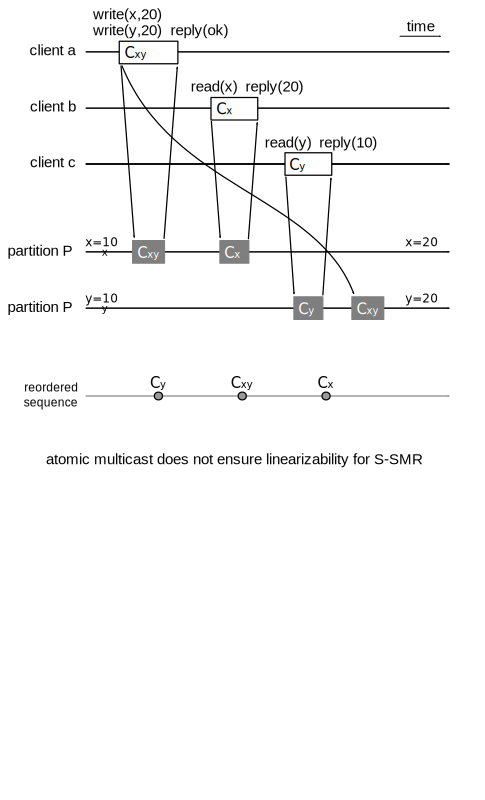
\includegraphics[width=0.9\columnwidth]{figures/mcastnonlinssmr} \\
%    \end{tabular}
%    \caption{Atomic multicast and S-SMR.}
%    \label{fig:mcastnonlinssmr}
%  \end{center}
%% \vspace{-4mm}
%\end{figure}
%
\begin{figure*}
\begin{minipage}[b]{1.0\linewidth} % A minipage that covers the whole width of the page
\centering
      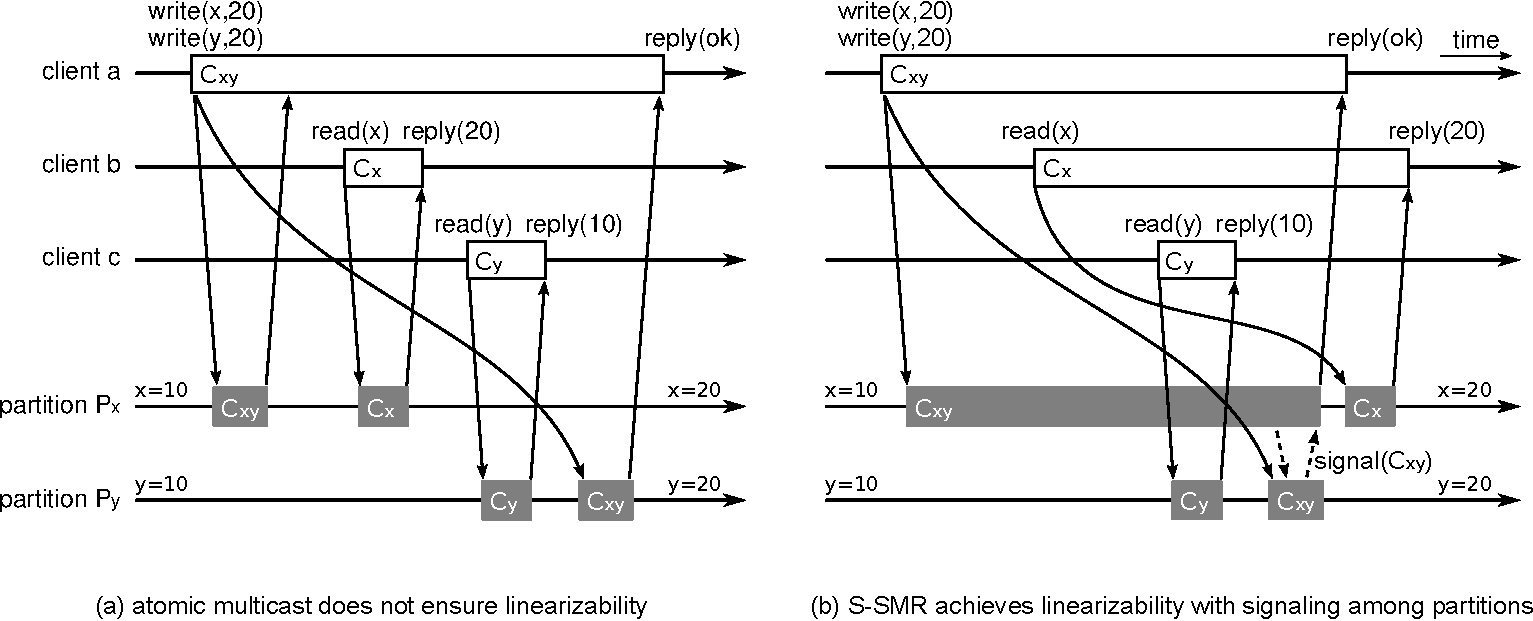
\includegraphics[width=0.85\linewidth]{figures/mcastssmr_nonlin_linsignal_v3}
\end{minipage}
%\begin{minipage}[b]{0.5\linewidth} % A minipage that covers half the page
%\centering
%      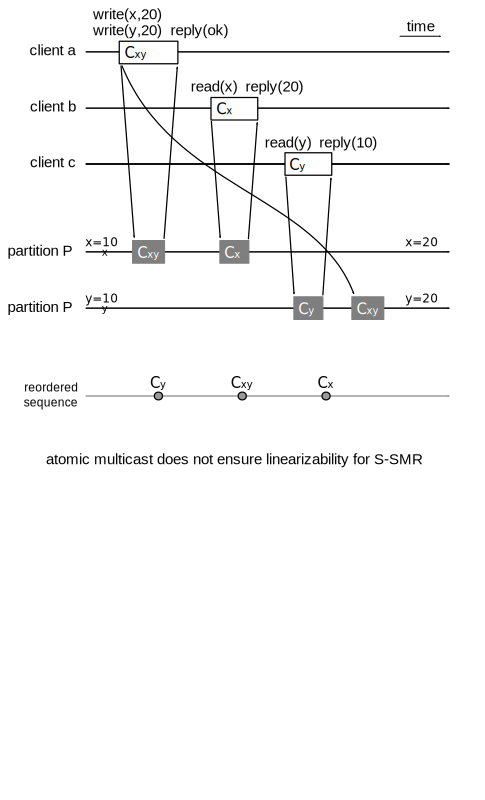
\includegraphics[width=0.9\columnwidth]{figures/mcastnonlinssmr}
%\end{minipage}
%\begin{minipage}[b]{0.5\linewidth}
%\centering
%      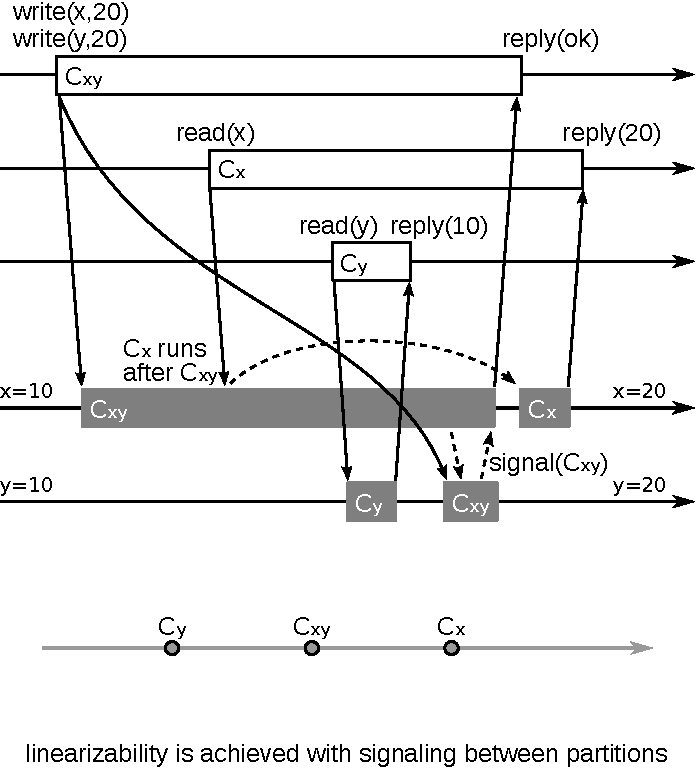
\includegraphics[width=0.9\columnwidth]{figures/mcastlinssmr_signal}
%\end{minipage}
\caption{Atomic multicast and S-SMR. (To simplify the figure, we show a single replica per partition.)}
\label{fig:mcastnonlinssmr}
\end{figure*}

Intuitively, the problem with the execution in Figure~\ref{fig:mcastnonlinssmr}~(a) is that commands $C_x$ and $C_y$ execute ``in between" the execution of $C_{xy}$ at partitions $\ppm_x$ and $\ppm_y$.
In S-SMR, we avoid such cases by ensuring that the execution of every command is atomic.
%
Command $C$ is \emph{execution atomic} if, for each server $s$ that executes $C$, there exists at least one server $r$ in every other partition in $part(C)$ such that the execution of $C$ at $s$ finishes after $r$ delivers $C$.
%
More precisely, let $delivery(C,s)$ and $end(C,s)$ be, respectively, the time when $s$ delivers command $C$ and the time when $s$ completes $C$'s execution.
Execution atomicity ensures that, for every server $s$ in partition \pp\ that executes $C$, there is a server $r$ in every $\ppm' \in part(C)$ such that $delivery(C,r) < end(C,s)$.
Intuitively, this condition guarantees that the execution of $C$ at $\ppm$ and $\ppm'$ overlap in time.

%Back in Fig.~\ref{fig:mcastnonlinssmr}, each black box represents the execution of a subcommand by servers in the partition: it starts when the first server in the partition begins executing the subcommand and ends when there is no more server executing the subcommand in that partition. We can see that $C_{xy}$ is not execution atomic: there is no time $t$ when some servers $s_x$ in $P_x$ and $s_y$ in $P_y$ are executing it. If it were the case, this example would be impossible to build, since $finish(C_y,s_y) < start(C_{xy}, s_y) < t < finish(C_{xy}, s_x) < start(C_x, s_x)$, which would contradict the fact that $C_x$ precedes $C_y$ in real-time.

Replicas can ensure execution atomicity by coordinating the execution of commands.
After delivering command $C$, servers in each partition send a $signal(C)$ message to servers in the other partitions in $part(C)$.
Before finishing the execution of $C$, each server must receive a $signal(C)$ message from at least one server in every other partition that executes $C$. 
%To minimize the waiting time to complete the execution of commands, servers may send such signal as soon as they deliver the command.
Moreover, if server $s$ in partition $\ppm$ receives the value of a variable from server $r$ in another partition $\ppm'$, as part of the execution of $C$, then $s$ does not need to receive a $signal(C)$ message from servers in $\ppm'$. This way, to tolerate $f$ failures, each partition requires $f+1$ servers; if all servers in a partition fail, service progress is not guaranteed.

Figure \ref{fig:mcastnonlinssmr}~(b) shows an execution of S-SMR. 
In the example, servers in $P_x$ wait for a signal from $P_y$, therefore delaying $C_{xy}$'s execution in $P_x$ and moving the execution of $C_x$ ahead in time. 
Note that the outcome of each command execution is the same as in case (a), but the executions of $C_x$, $C_y$ and $C_{xy}$, as seen by clients, now overlap in time with one another. 
Hence, there is no real-time precedence among them.

\subsection{Detailed algorithm}
\label{sec:detailalg}


\begin{algorithm}
\small
%\footnotesize
\begin{distribalgo}[1]
%\STATE \textbf{Algorithm 1:\\} Scalable State-Machine Replication (S-SMR)
\vspace{1mm}

\INDENT{\emph{Initialization:}}
    \STATE $\forall C \in \mathcal{K} : rcvd\_signals(C) \leftarrow \emptyset$
    \STATE $\forall C \in \mathcal{K} : rcvd\_variables(C) \leftarrow \emptyset$
\ENDINDENT

\vspace{1.5mm}
%\vspace{2.0mm}
\INDENT{\emph{Command $C$ is submitted by a client as follows:}}
    \STATE $dests \leftarrow oracle(C)$ \label{algline:oracle} 
%    \COMMENT{$oracle(C)$ returns a superset of $part(C)$}
	\STATE multicast$(dests, C)$ \label{algline:climcast}
	\STATE wait for response from one server
\ENDINDENT

\vspace{1.5mm}
%\vspace{2.0mm}
\INDENT{\emph{Command $C$ is executed by a server in partition \pp\ as follows:}}
	\INDENT{\textbf{upon} deliver$(C)$}
	    \STATE $others \leftarrow dests \setminus \{\ppm\}$ \label{algline:others}
	    \STATE multicast$(others, signal(C))$ \label{algline:mcastsignals}
		\FOR{each operation $op$ in $C$}
			\IF{$op$ is $read(v)$}
			    \IF{$v \in \ppm$}
			        \STATE multicast$(others, \{v,C.id\})$ \label{algline:multicastv}
			    \ELSE
			        \STATE \textbf{wait until} $v \in rcvd\_variables(C)$ \label{algline:waitvariable}
			        \STATE update $v$ with the value in $rcvd\_variables(C)$
			    \ENDIF
			\ENDIF
			\STATE execute $op$ \label{algline:executeopck}
		\ENDFOR
		\STATE \textbf{wait until} $rcvd\_signals(C) = others$ \label{algline:waitsignals}
		\STATE send reply to client \label{algline:sendreply}
	\ENDINDENT
	
	\vspace{2.0mm}
	\INDENT{\textbf{upon} deliver$(signal(C))$ from partition $\ppm'$}
	    \STATE $rcvd\_signals(C) \leftarrow rcvd\_signals(C) \cup \{\ppm'\}$
	\ENDINDENT

	\vspace{2.0mm}
	\INDENT{\textbf{upon} deliver$(\{v, C.id\})$}
	    \STATE $rcvd\_variables(C) \leftarrow rcvd\_variables(C) \cup \{v\}$
	\ENDINDENT
			
\ENDINDENT

\vspace{1.5mm}
%\vspace{2mm}

\textbf{Algorithm variables:}

\vspace{1mm}

$\mathcal{K}$: the set of all possible commands

\vspace{1mm}

$C.id$: unique identifier of command $C$

\vspace{1mm}

$oracle(C)$: function that returns a superset of $part(C)$

\vspace{1mm}

$dests$: set of partitions to which $C$ is multicast

\vspace{1mm}

$others$: set of partitions waiting for signals and variables from \pp; also, \pp\ waits for signals from all such partitions

\vspace{1mm}

$signal(C)$: a synchronization message that allows S-SMR to ensure $C$ to be execution atomic

\vspace{1mm}

$rcvd\_signals(C)$: a set containing all partitions that already signaled \pp\ regarding the execution of $C$

\vspace{1mm}

$rcvd\_variables(C)$: a set containing all variables that must be received from other partitions in order to execute $C$

\caption{Scalable State-Machine Replication (S-SMR)}
\label{alg:ssmr}
\end{distribalgo}
\end{algorithm}

In Algorithm \ref{alg:ssmr}, we show the basic operation of S-SMR. 
To submit a command $C$, the client queries an oracle to get set $dests$~(line \ref{algline:oracle}), which is a superset of $part(C)$ used by the client as destination set for $C$~(line \ref{algline:climcast}).

Upon delivering $C$, server $s$ in partition \pp\ multicasts $signal(C)$ to $others$, which is the set containing all other partitions involved in $C$ (lines \ref{algline:others} and \ref{algline:mcastsignals}). 
%The purpose of $signal(C)$ is to let servers in other partitions know that there is a server in \pp\ that started executing $C$. 
It might happen that $s$ receives signals concerning $C$ from other partitions even before $s$ started executing $C$. For this reason, $s$ must buffer signals and check if there are signals buffered already when starting the execution of $C$. For the sake of simplicity, Algorithm \ref{alg:ssmr} simply initializes such buffers as $\emptyset$ for all possible commands. In practice, buffers for $C$ are created when the first message concerning $C$ is delivered.

After multicasting signals, server $s$ proceeds to the execution of $C$, which is a sequence of operations that might read or write variables in \vv. The main concern is with operations that read variables, as they may determine the outcome of the command execution. All other operations can be executed locally at $s$. If the operation reads variable $v$ and $v$ belongs to \pp, $s$'s partition, then $s$ multicasts the value of $v$ to the other partitions that delivered $C$ (line \ref{algline:multicastv}). The command identifier $C.id$ is sent along with $v$ to make sure that the other partitions will use the appropriate value of $v$ during $C$'s execution. If $v$ belongs to some other partition $\ppm'$, $s$ waits until an up-to-date value of $v$ has been delivered (line \ref{algline:waitvariable}). Every other operation is executed with no interaction with other partitions (line \ref{algline:executeopck}).

After executing all operations of $C$, $s$ waits until a signal from every other partition has been received (line \ref{algline:waitsignals}) and, only then, sends the reply back to the client (line \ref{algline:sendreply}). This ensures that $C$ will be execution atomic.



\subsection{Performance optimizations}
\label{sec:optm}

Algorithm \ref{alg:ssmr} can be optimized in many ways. 
In this section, we briefly mention some of these optimizations and then detail caching.
\begin{itemize}
\item Server $s$ does not need to wait for the execution of command $C$ to reach a $read(v)$ operation to only then multicast $v$ to the other partitions in $part(C)$. If $s$ knows that $v$ will be read by $C$, $s$ can send $v$'s value to the other partitions as soon as $s$ starts executing $C$.
\item The exchange of objects between partitions serves the purpose of signaling. Therefore, if server $s$ sends variable $v$'s value to server $r$ in another partition, $r$ does not need to receive a signal message from $s$'s partition.
\item It is not necessary to exchange each variable more than once per command since any change during the execution of the command will be deterministic and thus any changes to the variable can be applied to the cached value.
\item Even though all replicas in all partitions in $part(C)$ execute $C$, a reply from a replica in a single partition suffices for the client to finish the command.
\end{itemize}

%Caching is a more elaborate optimization. 
Server $s$ in partition \pp\ can cache variables that belong to other partitions. 
There are different ways for $s$ to maintain cached variables; here we define two techniques: conservative caching and speculative caching. 
In both cases, the basic operation is the following: 
When $s$ executes a command that reads variable $x$ from some other partition $\ppm{}_x$, after retrieving the value of $x$ from a server in $\ppm{}_x$, $s$ stores $x$'s value in its cache and uses the cached value in future read operations.
If a command writes $x$, $s$ updates (or creates) $x$'s local value. 
Server $s$ will have a valid cache of $x$ until (i)~$s$ discards the entry due to memory constraints, or (ii)~some command not multicast to \pp\ changes the value of $x$. 
Since servers in $\ppm_x$ deliver all commands that access $x$, these servers know when any possible cached value of $x$ is stale.
How servers use cached entries distinguishes conservative from speculative caching.
%; what it does not know, however, is whether \pp\ has discarded $x$'s cache. 


Servers in $\ppm_x$ can determine which of its variables have a stale value cached in other partitions. This can be done by checking if there was any command that updated a variable $x$ in $\ppm_x$, where such command was not multicast to some other partition $\ppm$ that had a cache of $x$. Say servers in $\ppm_x$ deliver command $C$, which reads $x$, and say the last command that updated the value of $x$ was $C_w$. Since $x \in \ppm_x$, servers in $\ppm_x$ delivered $C_w$. One way for servers in $\ppm_x$ to determine which partitions need to update their cache of $x$ is by checking which destinations of $C$ did not receive $C_w$. This can be further optimized: even if servers in $\ppm$ did not deliver $C_w$, but delivered some other command $C_r$ that reads $x$ and $C_r$ was ordered by multicast after $C_w$, then $\ppm$ already received an up-to-date value of $x$ (sent by servers in $\ppm_x$ during the execution of $C_r$). If servers in $\ppm$ discarded the cache of $x$ (e.g., due to limited memory), they will have to send a request for its value.


\emph{Conservative caching}: Once $s$ has a cached value of $x$, before it executes a $read(x)$ operation, it waits for a cache-validation message from a server in $\ppm_x$. The cache validation message contains a set of pairs $(var, val)$, where $var$ is a state variable that belongs to $\ppm_x$ and whose cache in $\ppm$ needs to be validated. 
If servers in $\ppm_x$ determined that the cache is stale, $val$ contains the new value of $var$; otherwise, $\perp$, telling $s$ that its cached value is up to date.
If $s$ discarded its cached copy, it sends a request for $x$ to $\ppm_x$.
If it is possible to determine which variables are accessed by $C$ before $C$'s execution, all such messages can be sent upon delivery of the command, reducing waiting time; messages concerning variables that could not be determined a-priori are sent later, during the execution of $C$, as variables are determined.

\emph{Speculative caching}: It is possible to reduce execution time by speculatively assuming that cached values are up-to-date. 
Speculative caching requires servers to be able to rollback the execution of commands, in case the speculative assumption fails to hold. 
Many applications allow rolling back a command, such as databases, as long as no reply has been sent to the client for the command yet. 
The difference between speculative caching and conservative caching is that in the former servers that keep cached values do not wait for a cache-validation message before reading a cached entry; instead, a $read(x)$ operation returns the cached value immediately. 
If after reading some variable $x$ from the cache, during the execution of command $C$, server $s$ receives a message from a server in $\ppm_x$ that invalidates the cached value, $s$ rolls back the execution to some point before the $read(x)$ operation and resumes the command execution, now with the up-to-date value of $x$. 
%This may happen for every variable read by $C$, so $s$ might rollback the execution of $C$ several times until getting it right. 
%To ensure that a correct execution will be done eventually, 
Server $s$ can only reply to the client that issued $C$ after every variable read from the cache has been validated.

%Both caching algorithms depend on the following condition: each partition $\ppm_x$ keeps track of what was the last command $C$ executed by each partition $\ppm$, for each variable $x$ in $\ppm_x$, such that $C$ reads or writes $x$.\fixme{This part is too complicated.}
%Such values are kept by $\ppm_x$ in a table where each entry is $\langle \ppm, x, k \rangle$, where $k$ identifies the last command executed by $\ppm$ that accesses $x$. The initial value of $k$ is $0$ for every partition and every variable. Whenever a command $C$ that accesses $x$ is delivered by $\ppm_x$, it increments the command counter $k$ in $\langle \ppm, x, k \rangle$, for every partition $\ppm$ that delivers $C$. Upon delivery of any command $C'$ that also accesses $x$, $\ppm_x$ checks whether there is any partition $\ppm'$ that $C'$ was multicast to, where the cache of $x$ read by $C'$ will be stale, that is, entries $\langle \ppm_x, x, k \rangle$ and $\langle \ppm', x, k' \rangle$ are such that $k' < k$. Then, $P_x$ sends the cache-validation message(s) to $\ppm'$ accordingly.

\subsection{Correctness}
\label{sec:correctness}

In this proof, we denote the order given by atomic multicast with ``$\prec$''. Given any two messages $m_1$ and $m_2$, ``$m_1 \prec m_2$'' means that both messages are delivered by the same group and $m_1$ is delivered before $m_2$, or there is some message $m'$ such that $m_1 \prec m'$ and $m' \prec m_2$, which can be written as \mbox{$m_1 \prec m' \prec m_2$}.

We argue that, if every command in execution \ex\ of \mbox{S-SMR} is execution atomic, then \ex\ is linearizable. Suppose, by means of contradiction, that there exist two commands $x$ and $y$, where $x$ finishes before $y$ starts, but $y \prec x$ in the execution. There are two possibilities for this: (i) $x$ and $y$ access some variable in common $v$, or (ii) $x$ and $y$ access no variable in common.

In case (i), at least one partition $P_v$ (which contains $v$) delivers both $x$ and $y$. As $x$ finishes before $y$ starts, then $P_v$ delivers $x$, then $y$. From the properties of atomic multicast, and since each partition is mapped to a multicast group, no partition delivers $y$, then $x$. Moreover, atomic multicast ensures acyclic order, so there are no commands $z_1, ..., z_n$ such that their atomic order is $y \prec z_1 \prec \cdots \prec z_n \prec x$. So, we reached a contradiction in this case.

In case (ii), if there were no other command in \ex, then the execution of $x$ and $y$ could be done in any order, which would contradict the supposition that $y \prec x$. Therefore, there are commands $z_0, ..., z_n$ such that their atomic order is $y \prec z_0 \prec \cdots \prec z_n \prec x$. As $y \prec z_0$, then some partition $P_y$ delivers $y$, then $z_0$. Also, since $z_0 \prec z_1$, then some partition $P_1$ delivers $z_0$, then $z_1$, and so on: partition $P_i$ delivers $z_{i-1}$, then $z_i$, where $i \in \{1, ..., n\}$. Finally, partition $P_x$ delivers $z_n$, then $x$.

We now claim that for every $R_x \in P_x$, $R_x$ finishes executing $x$ only after some $R_0 \in P_0$ delivered $z_0$.
We prove our claim by induction.

Induction basis: As $z_n \prec x$, every $R_x \in Px$ executes command $x$ only after the execution of $z_n$ at $R_x$ finished. As $z_n$ is execution atomic, for every $R_x \in P_x$, there is a server $R_n \in P_n$ that delivered $z_n$ before $R_x$ finished executing $z_n$, which was before $R_x$ even started executing command $x$. Therefore, every $R_x \in P_x$ finishes executing $x$ only after some $R_n \in P_n$ delivered $z_n$.

Induction step: Assume that every $R_x \in P_x$ finishes executing $x$ only after some $R_i \in P_i$ delivered $z_i$. As $z_i$ is execution atomic, there is some $R_{i-1} \in P_{i-1}$ that delivered $z_i$ before $R_i$ finished executing $z_i$. As $z_{i-1} \prec z_i$ and $R_{i-1}$ delivers both, then $R_{i-1}$ delivers $z_{i-1}$ before executing $z_i$. Thus, $R_x \in P_x$ finishes executing $x$ only after some $R_{i-1}$ has delivered $z_{i-1}$, for every $R_x \in P_x$. This proves our claim.

Finally, for every $R_0 \in P_0$, there is a server $R_y \in P_y$ that delivers $z_0$ before $R_0$ finishes executing $z_0$. Since every $R_y$ delivers and executes $y$, then $z_0$, and from the claim above, for every $R_x \in P_x$, there is an $R_y \in P_y$ that delivers $y$ before $R_x$ finishes executing $x$. This contradicts the assumption that $x$ precedes $y$ in real-time, i.e., that the reply to $x$ is received before $y$ is invoked by a client.

% THE ALTERNATIVE BELOW ENDED UP EVEN MORE COMPLICATED!!!

% x = C_n
% y = C_1

%In this proof, we denote the order given by atomic multicast with ``$\prec$''. Given any two messages $m_1$ and $m_2$, ``$m_1 \prec m_2$'' means that both messages are delivered by the same group and $m_1$ is delivered before $m_2$, or there is some message $m'$ such that $m_1 \prec m'$ and $m' \prec m_2$, which can be written as \mbox{$m_1 \prec m' \prec m_2$}.
%
%We argue that, if every command in execution \ex\ of S-SMR is execution atomic, then \ex\ is linearizable. Suppose, by means of contradiction, that there exist two commands $C_1$ and $C_n$, where $C_1 \prec C_n$ in the execution, but $C_n$ finishes before $C_1$ starts. There are two possibilities for this: (i) $C_1$ and $C_n$ both access some variable in common $v$, or (ii) $C_1$ and $C_n$ access no variable in common.
%
%In case (i), at least one partition $P_v$ (which contains $v$) delivers both $C_1$ and $C_n$. As $C_n$ finishes before $C_1$ starts, then $P_v$ delivers $C_n$, then $C_1$. From the properties of atomic multicast, and since each partition is mapped to a multicast group, no partition delivers $C_1$, then $C_n$. Moreover, atomic multicast ensures acyclic order, so there are no commands $C_2, ..., C_{n-1}$ such that their atomic order is $C_1 \prec C_2 \prec \cdots \prec C_{n-1} \prec C_n$. So, we reached a contradiction in this case.
%
%In case (ii), if there were no other command in \ex, then there might be no partition that delivered both $C_1$ and $C_n$ and thus their execution could be done in any order, which would contradict the supposition that $C_1 \prec C_n$. Therefore, there are commands $C_2, ..., C_{n-1}$ such that their atomic order is $C_1 \prec C_2 \prec \cdots \prec C_{n-1} \prec C_n$. As $C_1 \prec C_2$, then some partition $P_1$ delivers $C_1$, then $C_2$. Also, since $C_2 \prec C_3$, then some partition $P_2$ delivers $C_2$, then $C_3$, and so on: partition $P_i$ delivers $C_i$, then $C_{i+1}$, where $i \in \{1, ..., n-1\}$.
%
%\textbf{Lemma}: For every server $R_{n-1} \in P_{n-1}$, $R_{n-1}$ finishes executing $C_n$ only after some server $R_1 \in P_1$ delivered $C_1$.
%
%We prove the proposition above by induction:
%
%Induction basis: As $C_{n-1} \prec C_n$, every $R_{n-1} \in P_{n-1}$ executes command $C_n$ only after the execution of $C_{n-1}$ at $R_{n-1}$ has finished. As $C_{n-1}$ is execution atomic, for every $R_{n-1} \in P_{n-1}$, there is a server $R_{n-2} \in P_{n-2}$ that delivered $C_{n-2}$ before $R_{n-1}$ finished executing $C_{n-1}$, which was before $R_{n-1}$ even started executing command $C_n$. Therefore, every $R_{n-1} \in P_{n-1}$ finishes executing $C_n$ only after some $R_{n-2} \in P_{n-2}$ started executing $C_{n-1}$.
%
%Induction step: Assume that every $R_x \in P_x$ finishes executing $x$ only after some $R_i \in P_i$ started executing $z_i$. As $z_i$ is execution atomic, there is some $R_{i-1} \in P_{i-1}$ that started execution $z_i$ before $R_i$ finished executing $z_i$. As $z_{i-1} \prec z_i$ and $R_{i-1}$ delivers both, then $R_{i-1}$ starts executing $z_{i-1}$ before executing $z_i$. Thus, $R_x \in P_x$ finishes executing $x$ only after some $R_{i-1}$ started executing $z_{i-1}$, for every $R_x \in P_x$. This proves Lemma 1.
%
%Finally, for every $R_0 \in P_0$, there is a server $R_y \in P_y$ that starts executing $z_0$ before $R_0$ finishes executing $z_0$. Since every $R_y$ delivers and executes $y$, then $z_0$, and from Lemma~1, for every $R_x \in P_x$, there is an $R_y \in P_y$ that starts executing $y$ before $R_x$ finishes executing $x$. This contradicts the assumption that $x$ precedes $y$ in real-time, i.e., that the reply to $x$ is received before $y$ is invoked by a client.
%
